% !TeX spellcheck = fr_FR
\chapter{Chapitre 3 : Communication PC - FPGA}

\section{Description Solution UART}

\subsection{Encodage Cobs}

Votre texte, votre texte, votre texte, votre texte, votre texte, votre texte, votre texte, votre texte, votre texte, votre texte, votre texte, votre texte, votre texte, votre texte, votre texte, votre texte, votre texte, votre texte.

\subsection{CRC}

Votre texte, votre texte, votre texte, votre texte, votre texte, votre texte, votre texte, votre texte, votre texte, votre texte, votre texte, votre texte, votre texte, votre texte, votre texte, votre texte, votre texte, votre texte.

\subsection{Transmission et Réception de Paquet}

\begin{figure}[tbph!]
	\centering
	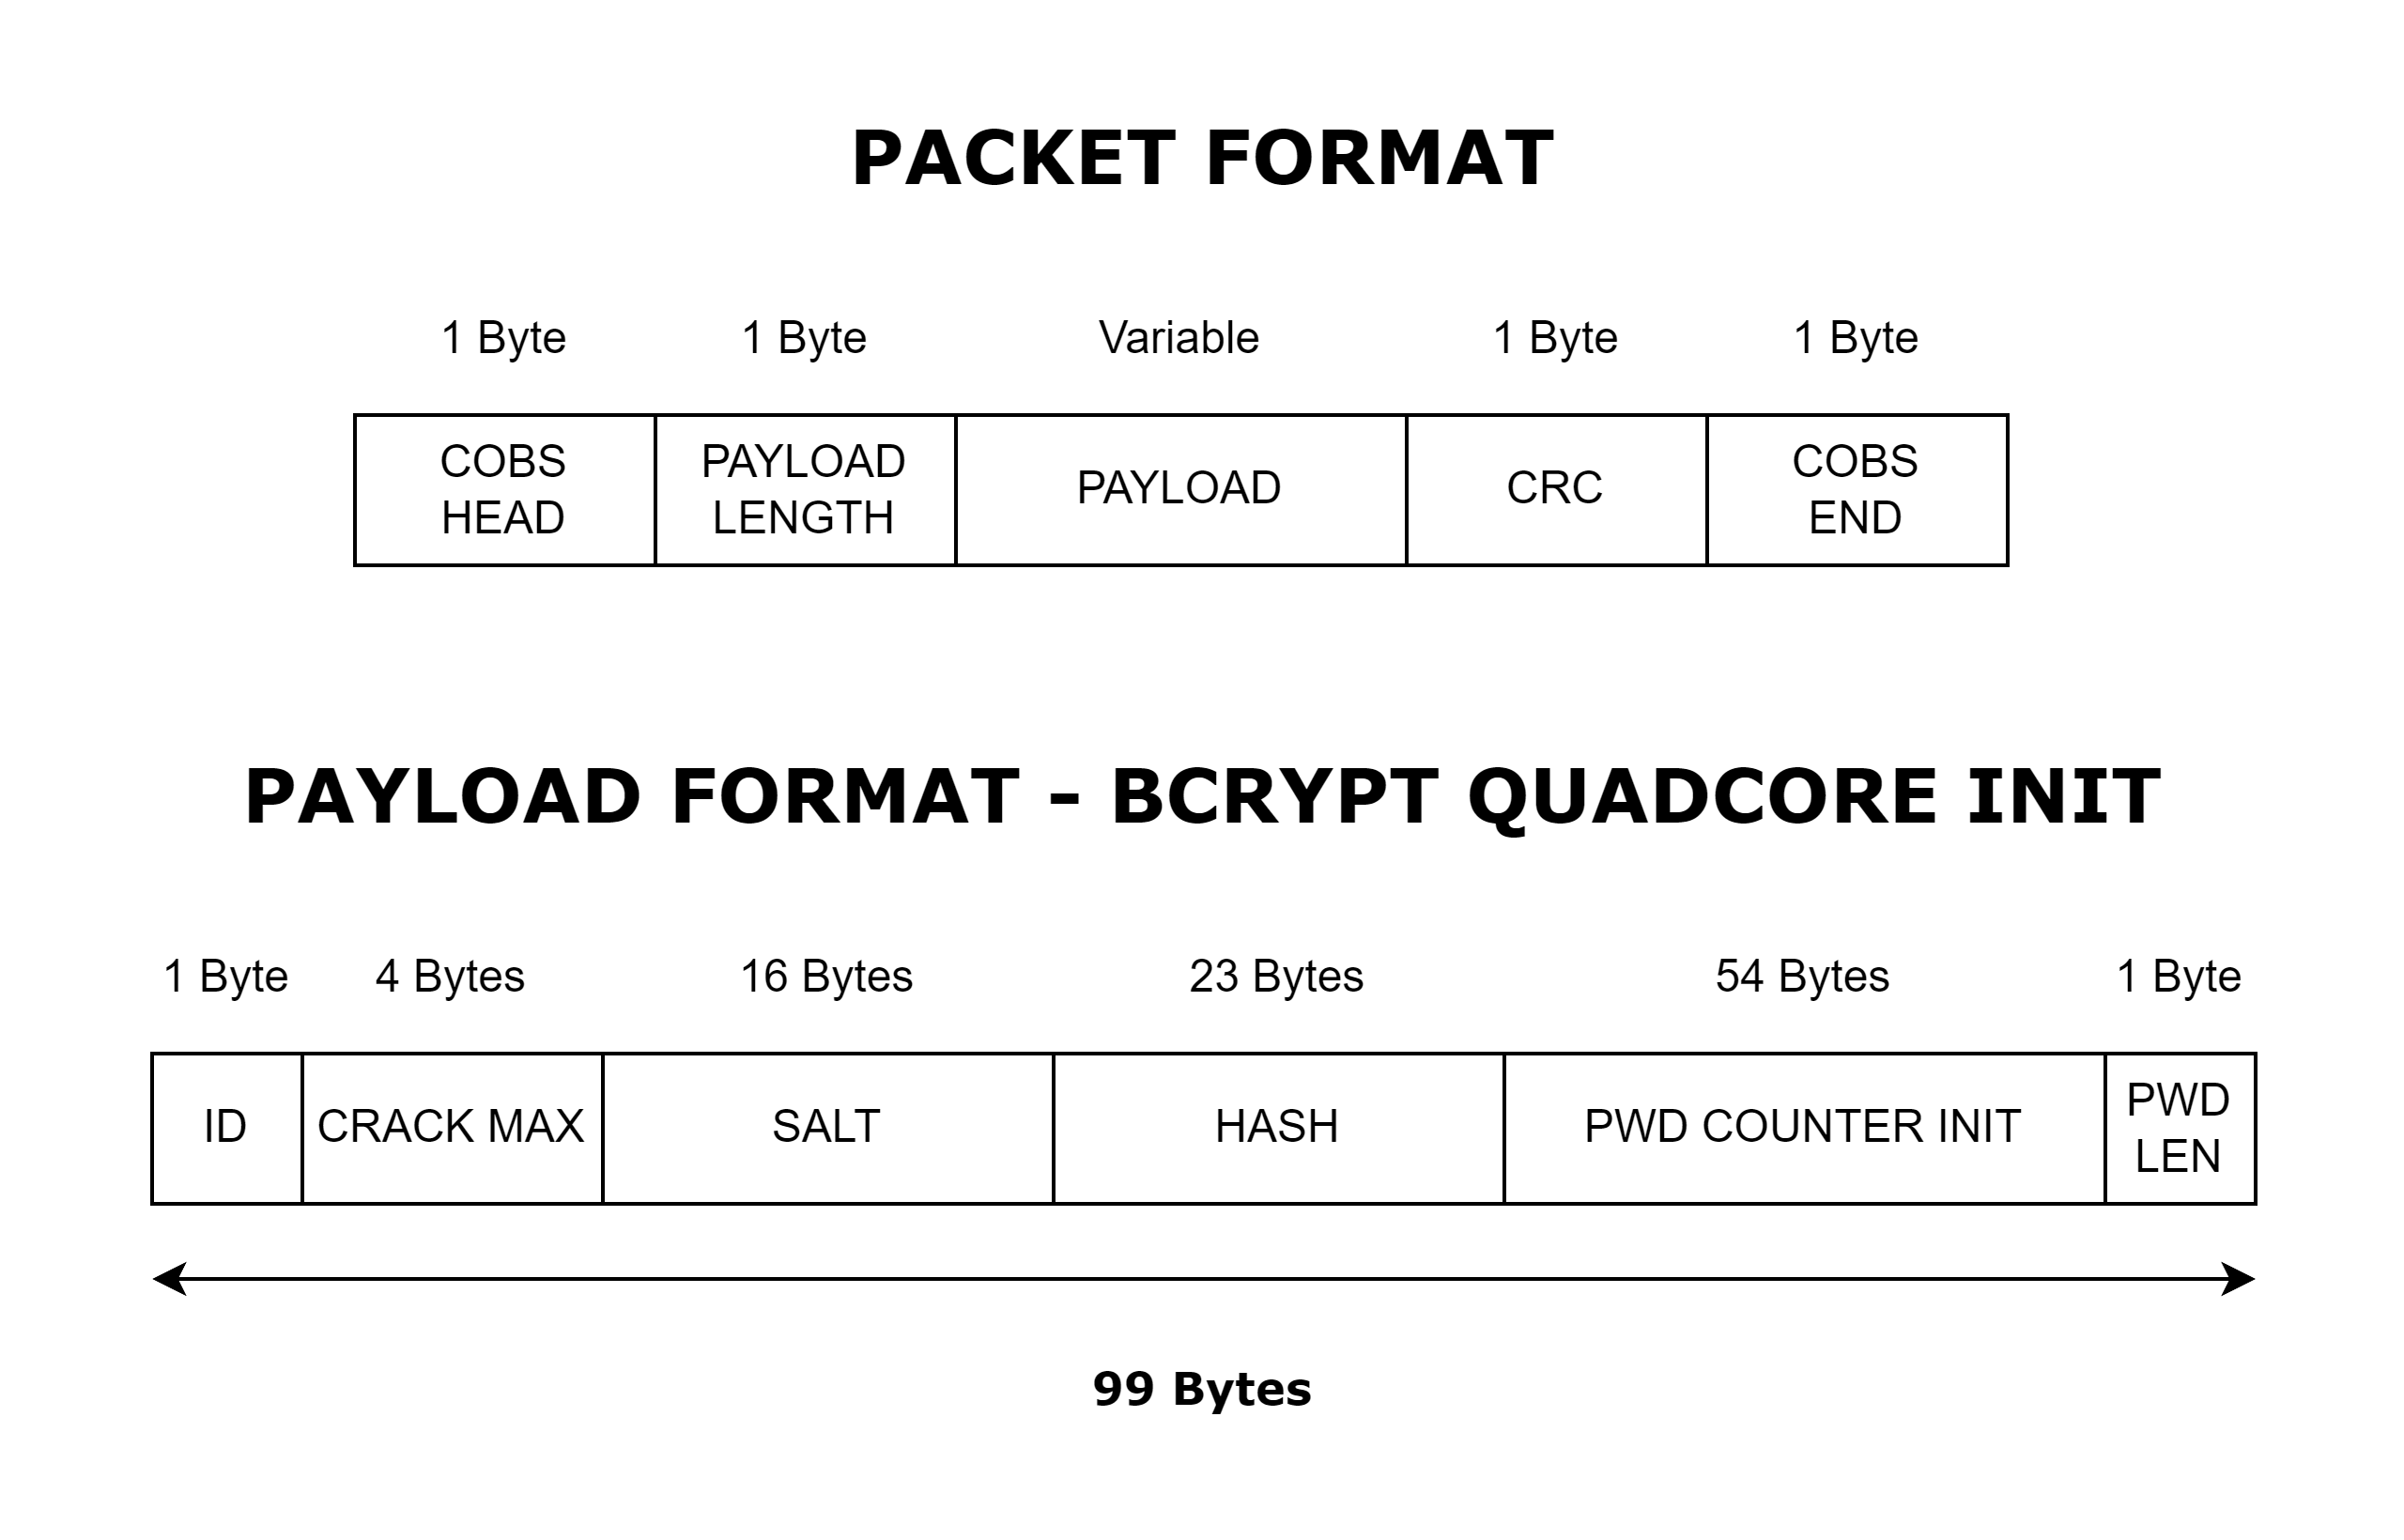
\includegraphics[width=0.7\linewidth]{communication_protocol_mosi_packet_format}
	\caption[Format de paquet - MOSI]{Format de paquet. Source : réalisé par Kandiah Abivarman}
	\label{fig:mosi_packet_format}
\end{figure}

\newpage

\begin{figure}[tbph!]
	\centering
	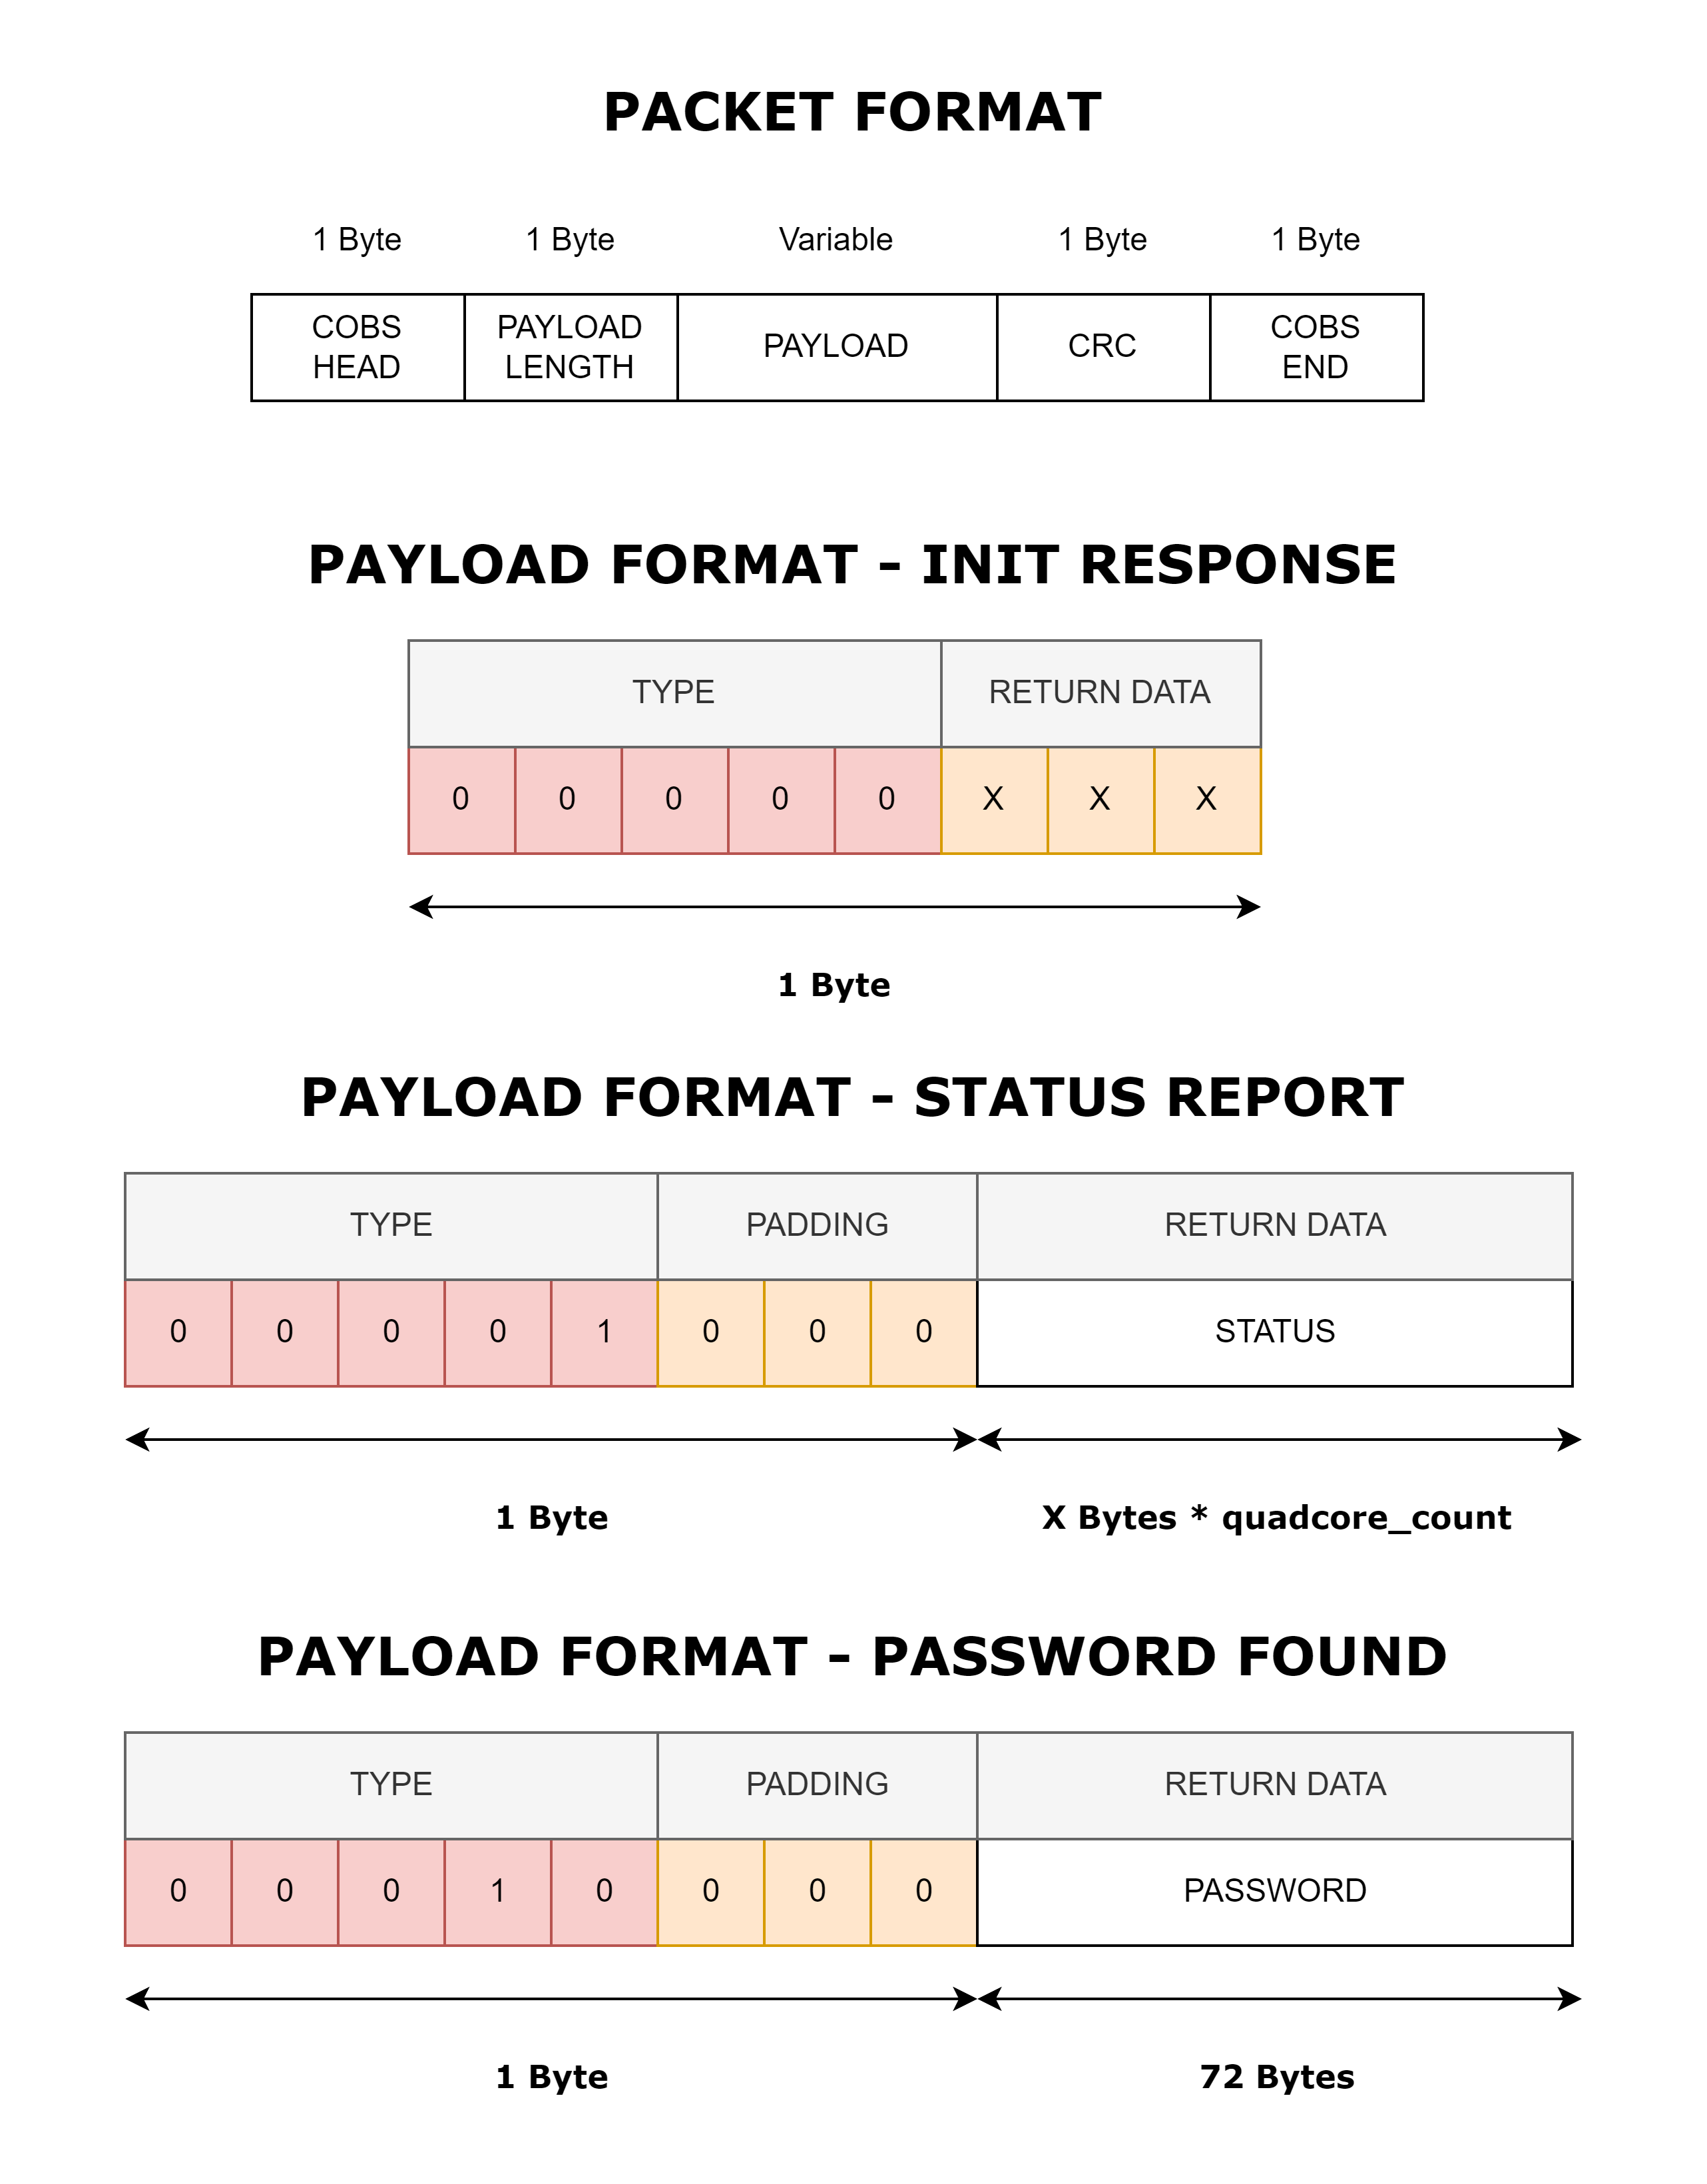
\includegraphics[width=0.7\linewidth]{communication_protocol_miso_packet_format}
	\caption[Format de paquet - MISO]{Format de paquet. Source : réalisé par Kandiah Abivarman}
	\label{fig:miso_packet_format}
\end{figure}

\newpage

\section{Implémentation Solution UART}

\subsection{Architecture Logique}

\begin{figure}[tbph!]
	\centering
	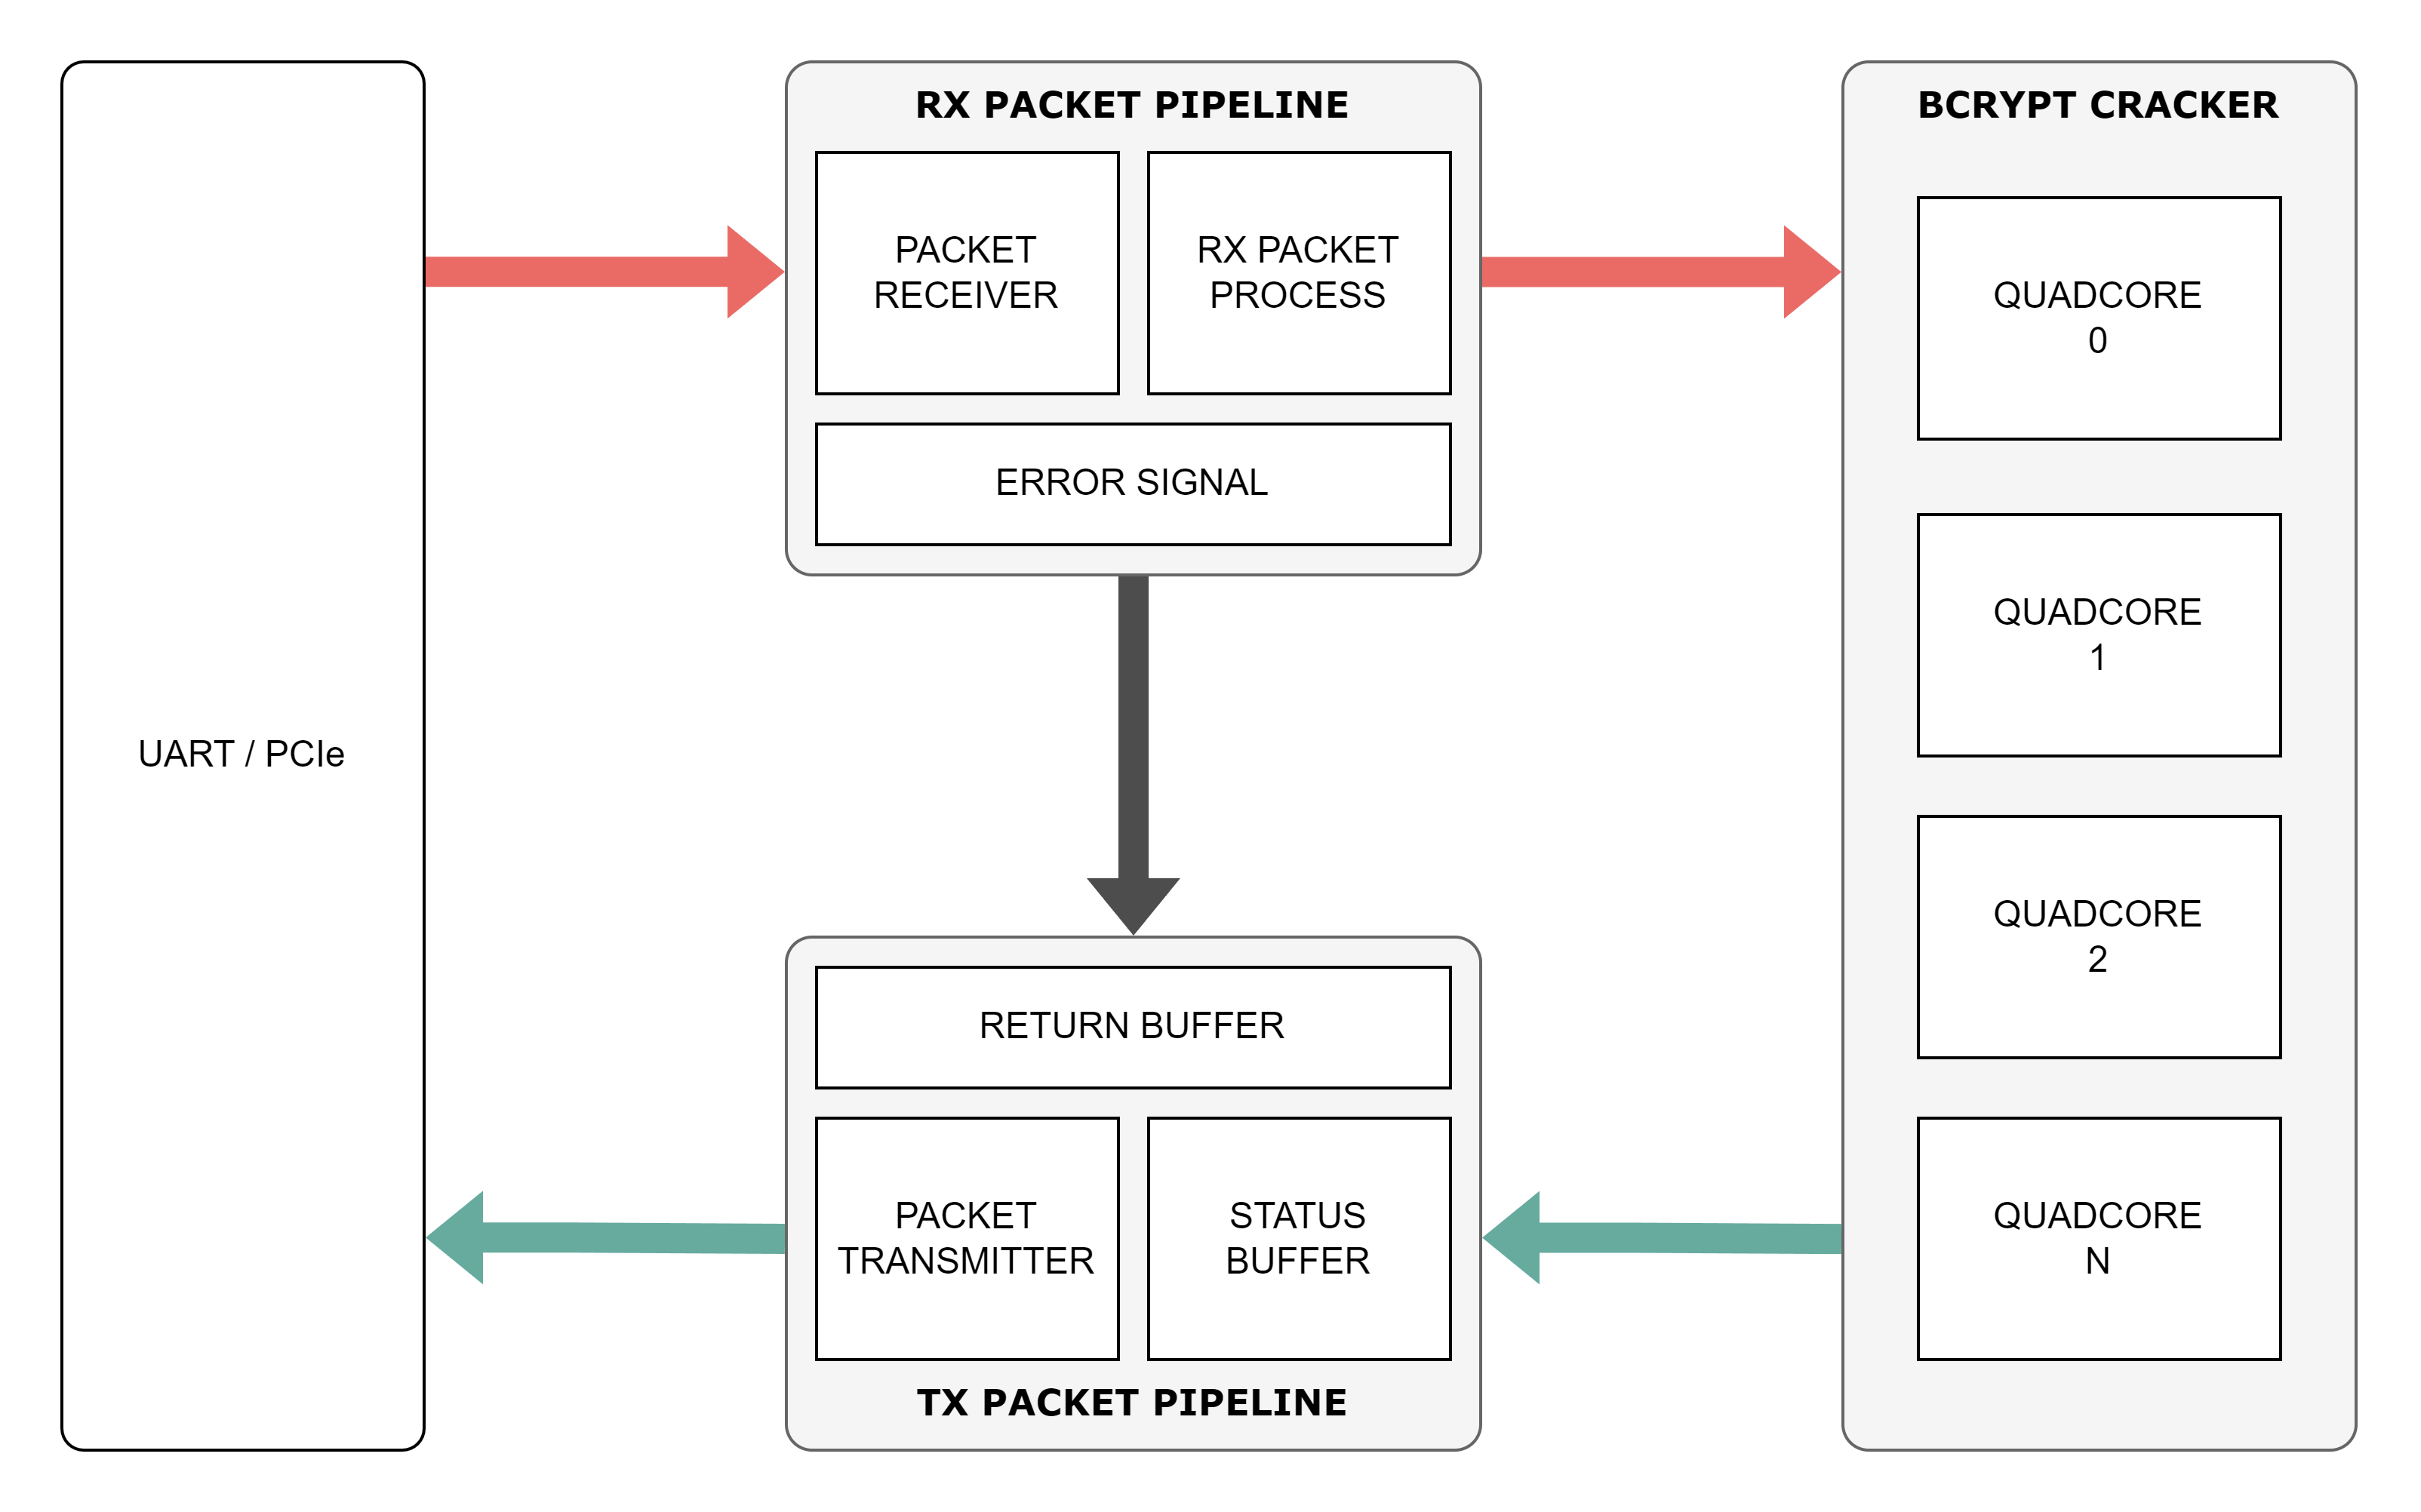
\includegraphics[width=0.7\linewidth]{communication_protocol_top_rev2}
	\caption[Schéma système UART - FPGA]{Schéma système UART. Source : réalisé par Kandiah Abivarman}
	\label{fig:uart_top_schematics}
\end{figure}

\subsection{UART}

\subsection{Modifications Bcrypt Cracker}

\subsection{Implémentation - MOSI}
\subsubsection{Module - Packet Receiver}
\subsubsection{Module - RX Packet Process}
\subsubsection{Module - RX Packet Pipeline}

\subsection{Implémentation - MISO}
\subsubsection{Module - Packet Transmitter}
\subsubsection{Module - TX Packet Pipeline}

\subsection{Tests}
\subsubsection{Simulations}
\subsubsection{Vérification Hardware}

\section{Interfacage Solution UART}

\newpage

\section{Description Solution PCIe}
\section{Implémentation Solution PCIe}
\section{Interfacage Solution PCIe}
